\newpage
\section{Example: Minesweeper}
In this section, we will develop a simple implementation of the well-known {\em Minesweeper} game.  Typically the minesweeper game is played through a graphical user interface, as illustrated by the following:
\begin{center}
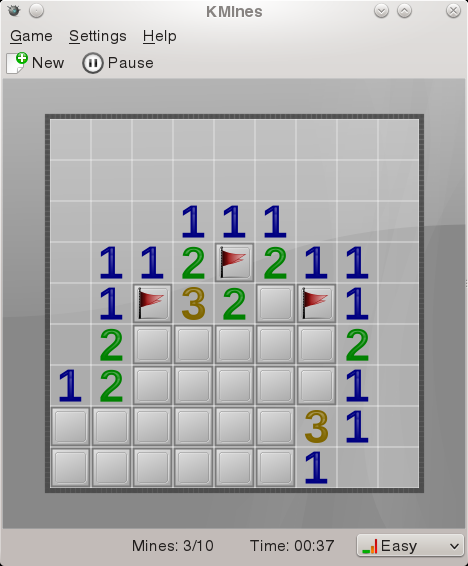
\includegraphics[width=0.4\textwidth]{../images/kmines.png}
\end{center}
Here, we can see the main aspects of the game.  The {\em game board} is a two-dimensional grid of {\em squares}.  Each square holds {\em nothing} or a {\em bomb} and is in one of the three states: {\em hidden}, {\em exposed} or {\em flagged} (with a flag).  An exposed square shows either the total number of bombs in the nine adjacent squares, or it shows a bomb (and the game is over).  Flagged squares are protected and cannot be exposed until they are unmarked.  The intuition here, is that the player marks those squares believed to contain a bomb.  Let us analyse the above board using the following diagram:

\begin{center}
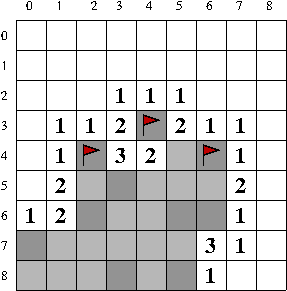
\includegraphics[width=0.4\textwidth]{../images/kmines_analysis.png}
\end{center}


The player plays the game by repeatedly selecting a square to expose.  When all squares are exposed, except for those containing bombs, the game is over and the player wins.  However, if a square holding a bomb is exposed, then the game is over immediately and the player loses.  A {\em blank} square is one with no adjacent bombs.  When a blank square is exposed, every adjacent blank square is recursively exposed.

